\documentclass{article}

\usepackage{graphicx}
\usepackage{tikz}
\usepackage{tikzsymbols}
\usetikzlibrary{calc,patterns,shapes.geometric}
\pagestyle{empty}
\usepackage[margin=0pt]{geometry}
\geometry{papersize={14in,12in}}

\def\centerarc[#1](#2)(#3:#4:#5){\draw[#1] ($(#2)+({#5*cos(#3)},{#5*sin(#3)})$) arc (#3:#4:#5);}

\begin{document}
	\begin{figure}
		\centering
		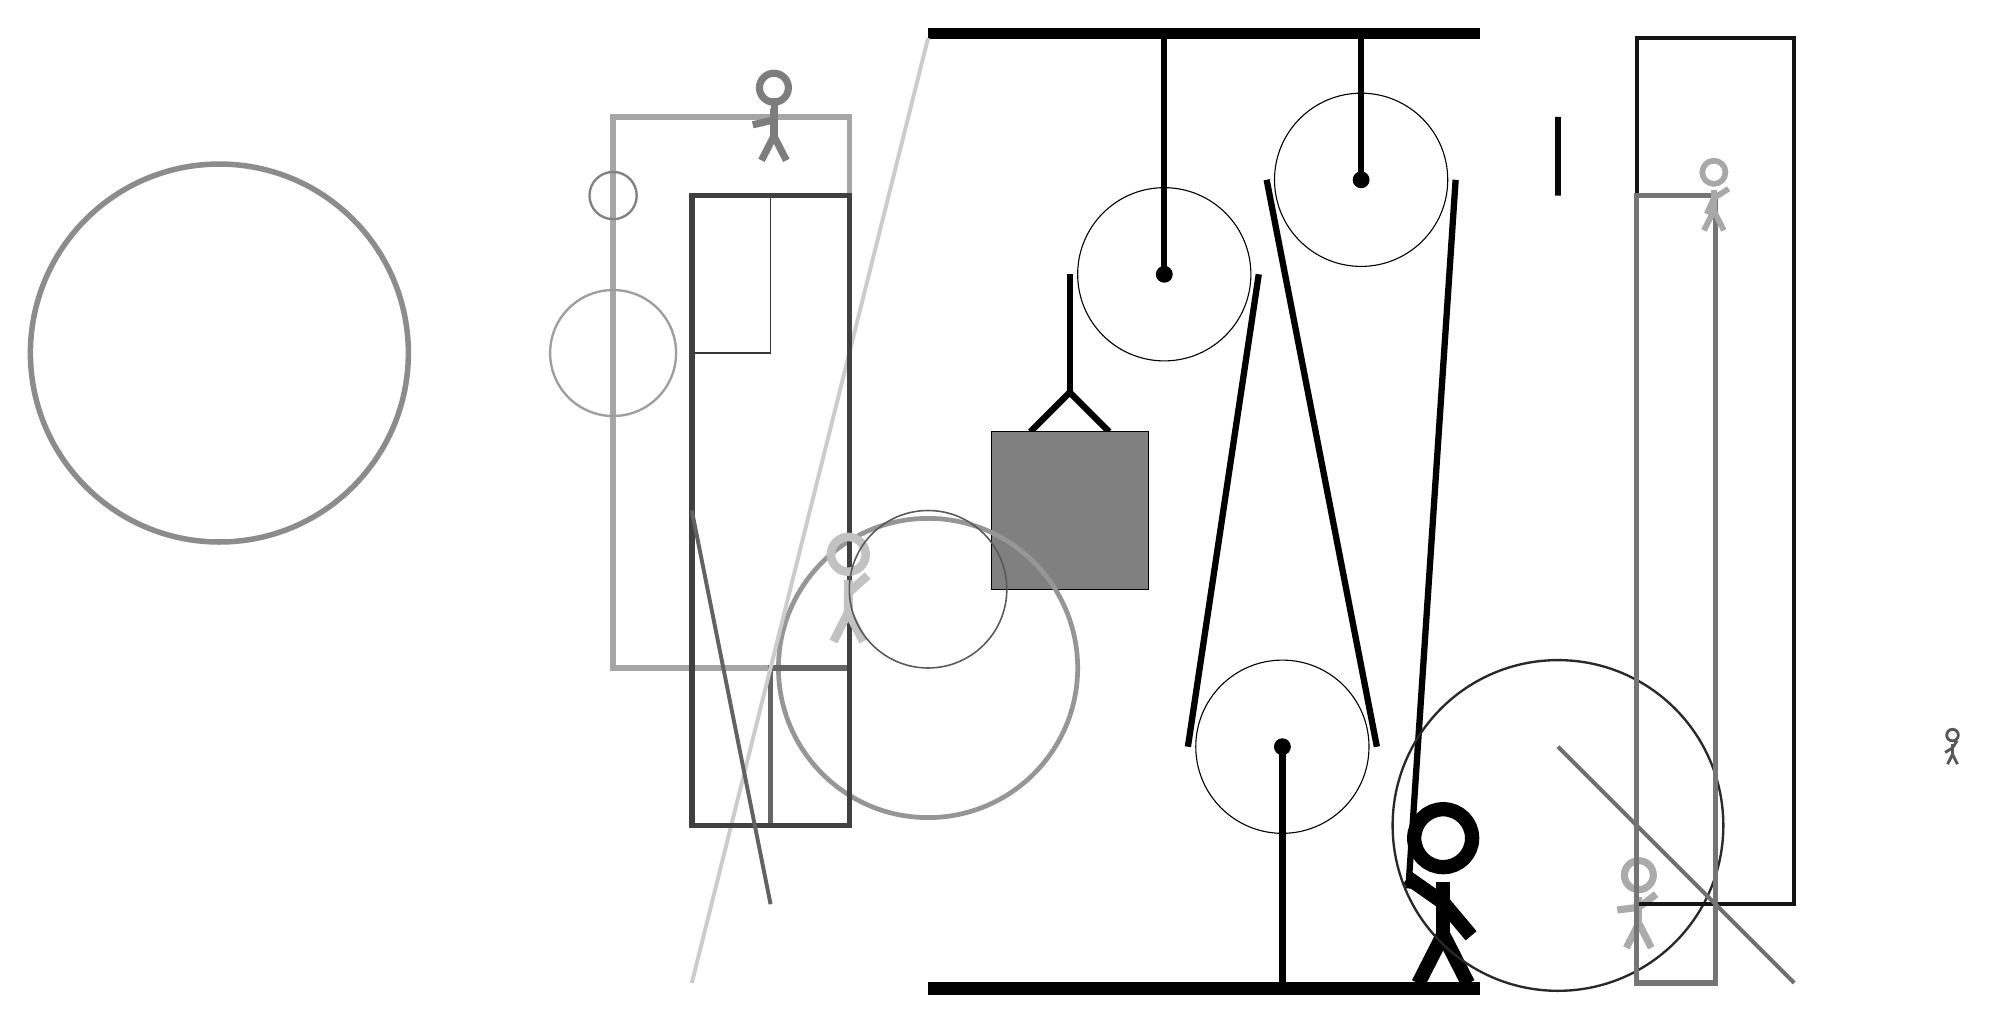
\begin{tikzpicture}
			%%%%% START %%%%%
			
			\draw[fill=black] (-2, 9) rectangle (5, 9.125);
			
			\draw (1, 6) circle (1.1);
			\draw[fill=black] (1, 6) circle (0.1);
			\draw[line width=0.8mm]  (1, 9) -- (1, 6);
			
			\draw[fill=white](2.5, 0) circle (1.1);
			\draw[fill=black] (2.5, 0) circle (0.1);
			\draw[line width=0.8mm]  (2.5, -3) -- (2.5, 0);
			
			\draw[fill=white](3.5, 7.2) circle (1.1);
			\draw[fill=black] (3.5, 7.2) circle (0.1);
			\draw[line width=0.8mm] (3.5, 9) -- (3.5, 7.2);
			
			\draw[line width=0.8mm] (-0.7, 4.0) -- (-0.2, 4.5) -- (0.3, 4.0);
			\draw[fill=black!50] (-1.2, 4.0) rectangle (0.8, 2.0);
			
			\draw[line width=0.8mm] (-0.2, 6) -- (-0.2, 4.5);
			\centerarc[line width=0.8mm](1, 6)(0:180:1.2000000000000002);
			\draw[line width=0.8mm](2.2, 6) -- (1.3, 0);
			\centerarc[line width=0.8mm](2.5, 0)(180:360:1.2000000000000002);
			\draw[line width=0.8mm](3.7, 0) -- (2.3, 7.2);
			\centerarc[line width=0.8mm](3.5, 7.2)(0:180:1.2000000000000002);
			\draw[line width=0.8mm](4.7, 7.2) -- (4.1, -1.8);
			
			\node at (4.5, -1.9) {\Strichmaxerl[10][-35][-50]};
			
			\node[line width=0.6mm, color=black!33] at (7, -2) {\Strichmaxerl[5][7][37]};
			
			\draw [line width=0.3mm, color=black!84](6, -1) circle (2.1);
			\draw [line width=0.7mm, color=black!45](-11, 5) circle (2.4);
			\draw[line width=0.7mm, color=black!35] (-3, 1) rectangle (-6, 8);
			\draw[line width=0.5mm, color=black!92] (7, 9) rectangle (9, -2);
			
			\draw[line width=0.5mm, color=black!56](6, 0) -- (9, -3);
			\draw [line width=0.6mm, color=black!41](-2, 1) circle (1.9);
			
			\node[line width=0.4mm, color=black!51] at (-4, 8) {\Strichmaxerl[5][13][88]};
			\draw [line width=0.3mm, color=black!49](-6, 7) circle (0.3);
			\draw[line width=0.7mm, color=black!60] (-4, 1) rectangle (-3, -1);
			\draw[line width=0.5mm, color=black!20](-5, -3) -- (-2, 9);
			\draw[line width=0.7mm, color=black!54] (7, -3) rectangle (8, 7);
			\draw [line width=0.3mm, color=black!38](-6, 5) circle (0.8);
			
			\draw[line width=0.7mm, color=black!97] (6, 8) rectangle (6, 7);
			\draw[line width=0.2mm, color=black!79] (-4, 7) rectangle (-5, 5);
			\node[line width=0.2mm, color=black!34] at (8, 7) {\Strichmaxerl[4][66][32]};
			
			\draw[line width=0.7mm, color=black!75] (-3, 7) rectangle (-5, -1);
			
			\node[line width=0.2mm, color=black!66] at (11, 0) {\Strichmaxerl[2][31][58]};
			\node[line width=0.5mm, color=black!24] at (-3, 2) {\Strichmaxerl[6][89][42]};
			\draw[line width=0.5mm, color=black!61](-4, -2) -- (-5, 3);
			\draw [line width=0.2mm, color=black!65](-2, 2) circle (1.0);
			
			\draw[fill=black] (-2, -3) rectangle (5, -3.15);
			
			%%%%% END %%%%%
		\end{tikzpicture}
	\end{figure}	
\end{document}